\chapter{車載センシング技術}
\section{車体モデル}
 車両と歩行者との衝突はまっすぐな道路上で起こることがほとんどであり,モデルを単純化するために直線運動のみを考慮した車両の車体モデルを図1に示す.\\
\newpage
\begin{figure}[H]
    \centering
    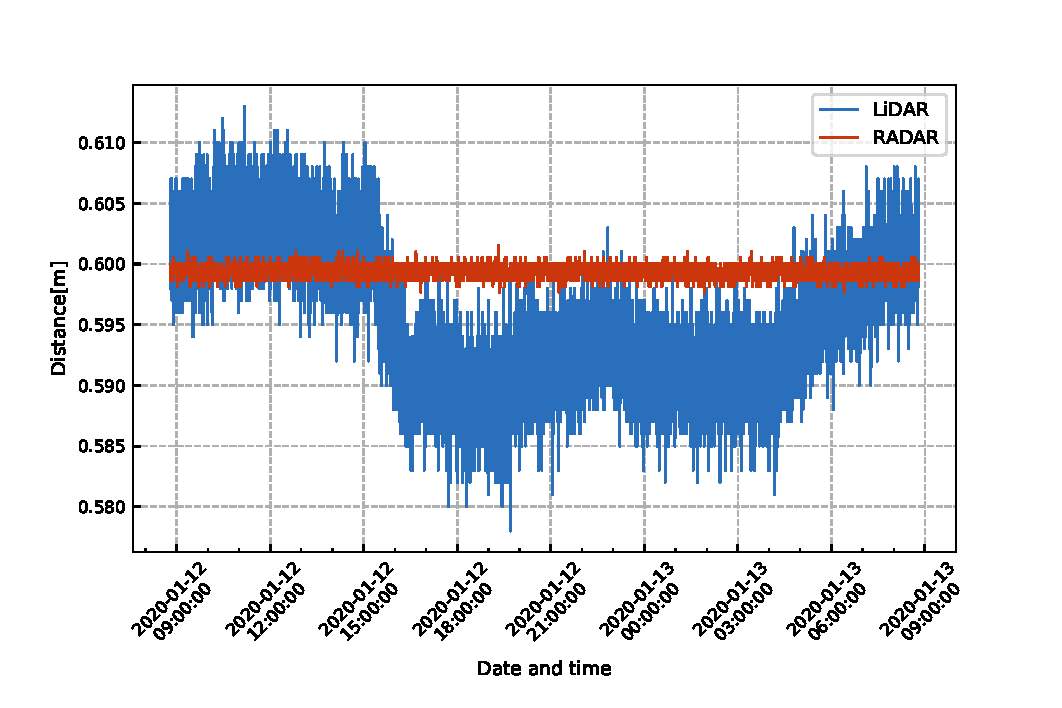
\includegraphics[width=12cm]{./fig/comparison_raw.pdf}
    \caption{LiDARとRADARの比較}
\end{figure}
\begin{figure}[H]
    \centering
    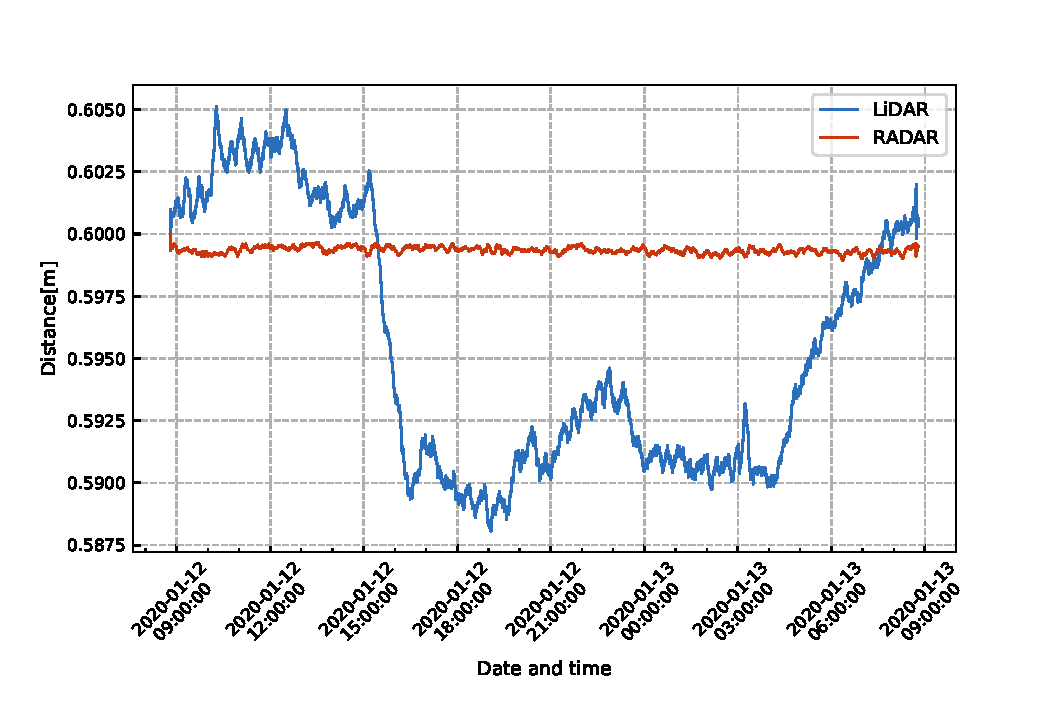
\includegraphics[width=12cm]{./fig/comparison_filtered60.pdf}
    \caption{フィルタ後}
\end{figure}



 図1に示すように,車両の車体の運動学とダイナミクスは次のとおり.\\
\begin{flalign}
    &\dot{x} = v\cos(\theta)\\
    &\dot{y} = v\sin(\theta)\\
    &M\dot{v} = nF_d+F_r
\end{flalign}

 ここで $x$ と $y$ は車両の位置である. $v$,$\theta$,$M$,$n$,$F_d$,$F_r$ は,それぞれ車速,車両角度,車両質量,制御輪数,駆動力,駆動抵抗である.$\Sigma$ はワールド座標系を表す.したがって,$\Sigma$ の $x$ と $y$ は,それぞれ緯度と経度の位置を示す.一般的に,抵抗力は移動方向に対して反対方向を向いている.ただし,駆動抵抗は正の値でも負の値でも構わない.この論文では,$F_r$ は $F_d$ と同じ方向を向いている.\\
 ちなみに,本論文の制御法にはモデル予測制御(MPC)を含んでおり,MPCは離散状態で定式化される.したがって,車体モデルの線形移動のみを制限した離散時間状態空間表現は,次のように表される.\\
\begin{flalign}
    &{\boldsymbol x}[k+1] = {\boldsymbol Ax}[k]+B(u[k]+F_r) ,\\
    &{\boldsymbol z} = {\boldsymbol Cx}[k]
\end{flalign}
なお
\begin{flalign}
    &A = \left[
        \begin{array}{rrr}
            1 & 0 & T_s\cos\theta \\
            0 & 1 & T_s\sin\theta \\
            0 & 0 & 1
        \end{array}
    \right]\nonumber\\
    &B = \left[
        \begin{array}{rrr}
            \frac{1}{2M}T_s^2\cos\theta & \frac{1}{2M}T_s^2\sin\theta & \frac{T_s}{M}
        \end{array}
    \right]^{\mathrm{T}}\nonumber
\end{flalign}
 ここで $T_s$ はサンプリング時間を表している. $u[k]$ は各車輪の力の合計であり,システムの出力変数は状態変数に等しい. これは, $x$,$y$,$v$に関する情報を取得できることを示している.日本では準天頂衛星システム(QZSS)などの測位技術の開発により,車両の位置を高精度に計測できるため,論文はこれらの値が得られると仮定している.

\section{ホイールモデル}
図2に示すホイールモデルのダイナミクスは次のように説明される.
\begin{figure}[h]
    \centering
    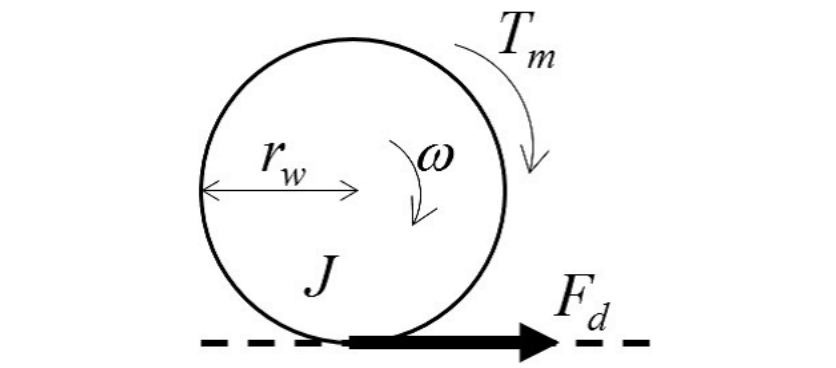
\includegraphics[width=8cm]{./fig/fig2.png}
    \caption{車両のホイールモデル}
\end{figure}

\begin{flalign}
    &J\dot{\omega} = T_m - r_m F_d\\
    &F_d = \mu(\lambda)\frac{Mg}{n}\\
    &\lambda = \frac{v-r_\omega\omega}{\mbox{max}(v,r_\omega\omega)}
\end{flalign}
ここで,$J$,$T_m$,$\omega$,$r_w$,$\lambda$および$\mu$は,それぞれモーターの慣性,モーターまたはブレーキ装置によって生成されるトルク,車輪角速度,車輪半径,スリップ率,および摩擦係数を表している. $\mu$はスリップ率$\lambda$の関数であり,$\mu$は法線力とタイヤ力の比を示していることに注意.

\section{摩擦円}
 摩擦円理論によれば,縦力Fxと横力Fyを含むタイヤ力は,式(9)となる.
\begin{equation}
    \sqrt{F^{x^{2}}+F^{y^{2}}} \leq \mu_{\max } M g
\end{equation}

 $\mu_{max}$は最大摩擦係数を示し,$g$は重力加速度である.式(9)は,縦力と横力の合力に上限があることを示している.合力が式の右側を超える場合,タイヤがスリップし,ドライバーが車両を制御できなくなる.したがって,スリップ現象を回避するためにはタイヤの力を制御する必要がある.